\section{Dataset}
\label{sec:data}
For aspect-based QA pairs generation, we provide a textual QA dataset with aspects for this task.
In this section, we will introduce the creation and analysis of this dataset.
%We provide a textual QA dataset with aspects, an evaluation metric and two baselines for this spect-based QA pairs generation task. 
%We will introduce the dataset and the evaluation metric in this section.
\subsection{Dataset Creation}
SQuAD2.0 is a well known textual QA dataset with the amount of annotated QA pairs from documents.
Therefore in this paper, we just add the aspect keywords for each paragraph of the SQuAD2.0 dataset to support our experiments.
\paragraph{Data Format}
The format of this aspect-based QA dataset is constructed as a quadruple $(Aspect, Context, Question, Answer)$.
The $Context$, $Question$ and $Answer$ are extracted from SQuAD 2.0, and for each $Question$, we only keep the first $Answer$.
For each quadruple, its QA pair is generated from the context and reflects the property or instance of the newly added $Aspect$.

\paragraph{Aspect Keywords Collection}
To allocate a suitable aspect keyword for each QA pair in SQuAD, 
we make an assumption that the QA pairs with the same context share the same aspect keywords, then 
convert the context to original Wikipedia pages and extract corresponding headings as the aspects.
In this step, to ensure that the paragraphs in SQuAD are consistent with the corresponding paragraphs in the original Wikipedia, 
we did not select wiki dumps as the source to obtain aspect keywords but crawled the most similar wiki texts which are distributed between 2012 and 2016.
To obtain the aspect keywords, we build a tree structure to represent each Wikipedia page.
The root node of the tree is the title of a Wikipedia page, the other non-leaf nodes from top to bottom are subheadings of different levels and the leaf nodes are the context of paragraphs.
After determining a leaf node by a given paragraph, we can find its root-to-leaf path, then we can remove the root node and leaf node and regard the content of other nodes as the aspect keywords of this paragraph.
Figure \ref{fig:wiki} shows an example of a Wikipedia page with the information followed by the aspect-based QA dataset.

\begin{figure*}[th]
    \begin{center}
    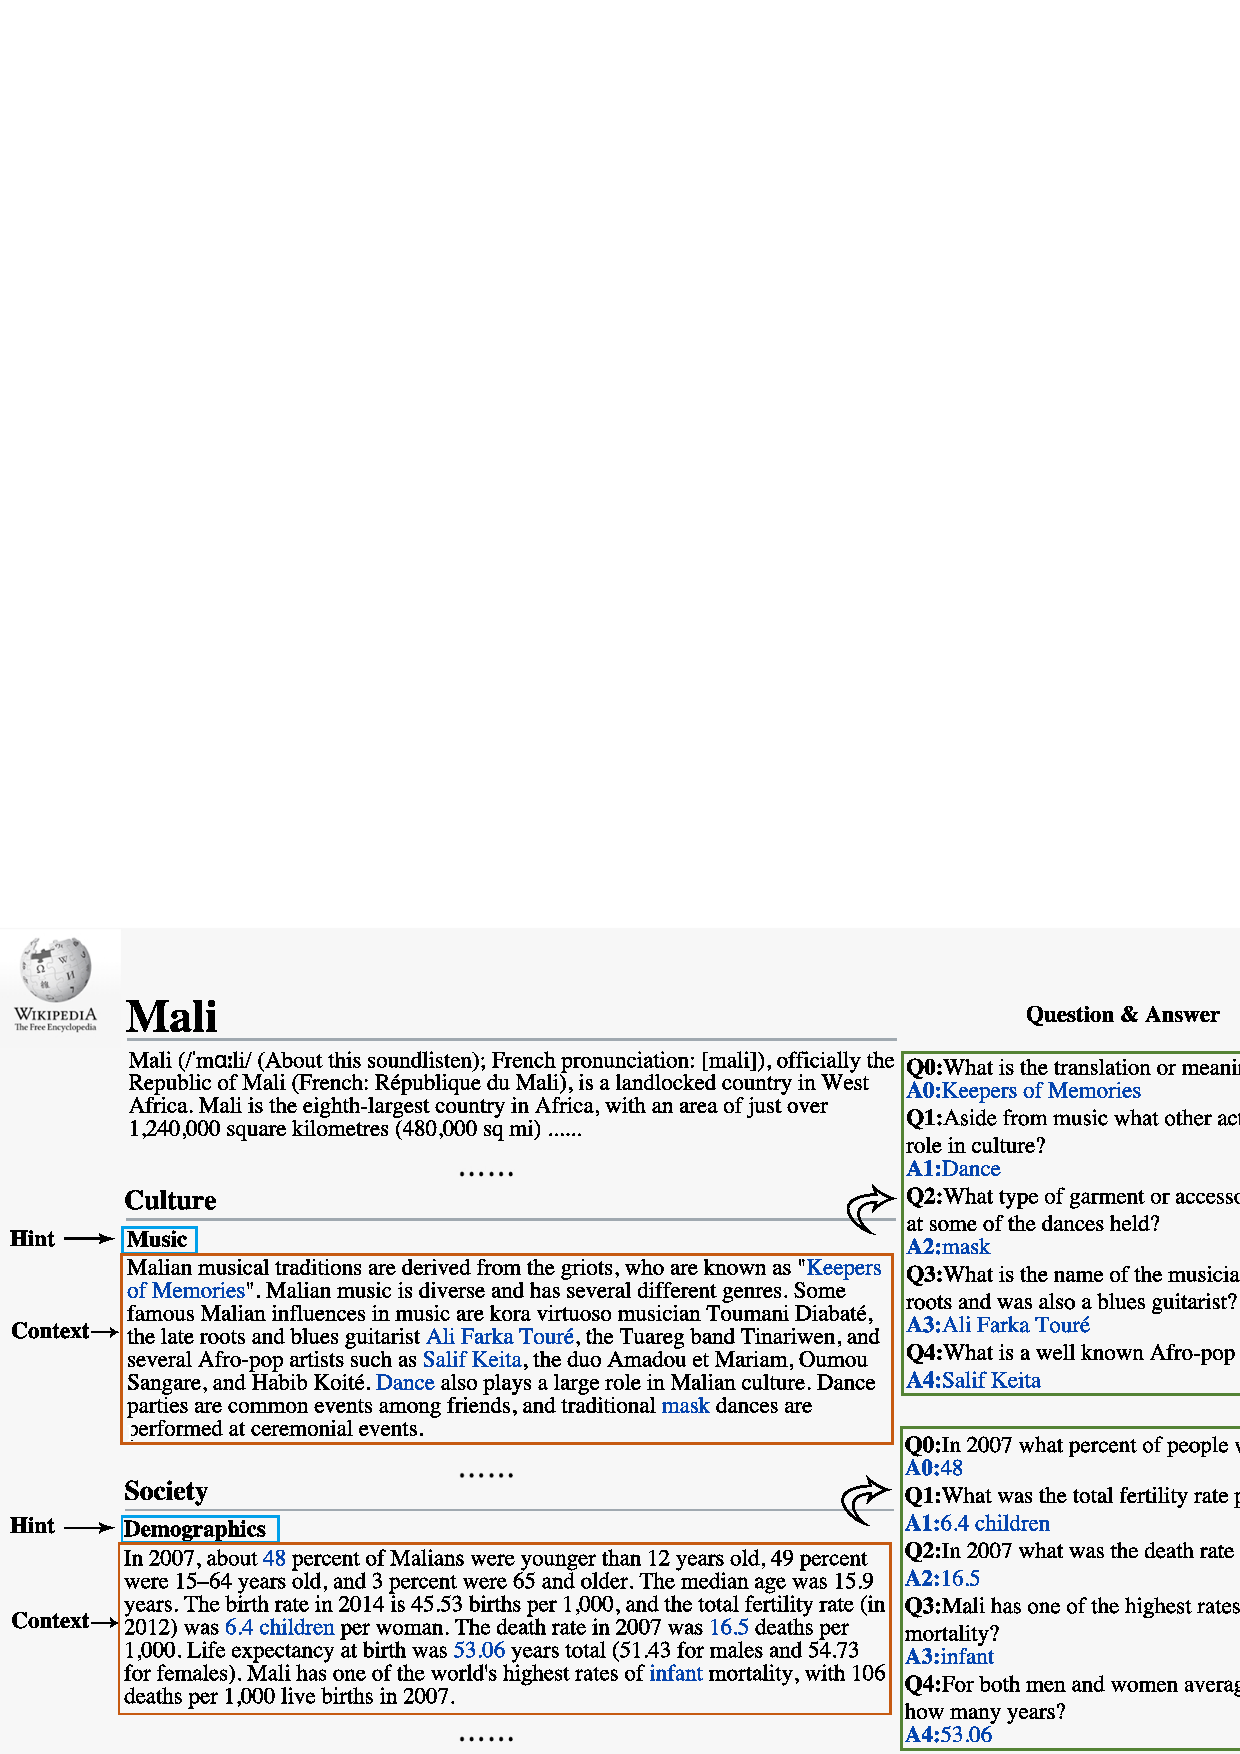
\includegraphics[width=0.8\textwidth]{pic/Wikipedia.pdf}
        \caption{\label{fig:wiki} An example of Wikipedia page \textbf{Black Death} and the information followed by our aspect-based QA dataset.
        The blocked context is the paragraph included in SQuAD2.0. The aspect keyword is the closest heading of the paragraph and the QA pairs on the right side are annotated in SQuAD2.0. The emoji in this figure is to show the relevance between the QA pairs and  aspect.}
    \end{center}
\end{figure*}

\subsection{Annotated Evaluation Set}
Although the paragraph is highly relevant to its aspect, not all of the QA pairs in SQuAD are related to this aspect.
The example in Figure \ref{fig:wiki} also shows this phenomenon. 
This paragraph talks about the causes of black death, in which QA1 and QA2 are relevant to this aspect.
However, QA0 is irrelevant which is talking about the details far from the topic.

We randomly select 100 QA pairs to judge whether they are relevant to their aspects, and find there are 60.58\% relevant samples.
%Due to the noise in our dataset, three master students are asked to label the relevance between the aspect keywords and the QA pairs.
%We assume that noisy samples are still aspect useful.
%To ensure sufficient training samples and , we only manually select the relevant test data to do the evaluation.
To ensure sufficient training data,
we assume that noisy samples are still aspect useful.
Then we use the noise data to train the QA generative models and manually select the relevant test data to do the evaluation.
For creating test data, three master students are asked to 
pick out the QA pairs that are really related to the aspect keywords.
%label the relevance between aspect keywords and the QA pairs.
%We provide the annotators with 368 paragraphs of the QA pairs with the crawled aspect candidates 
%and ask them to judge whether a QA pair is relevant to a given aspect keyword.
We provide the annotators with 3317 test quadruples and ask two of the annotators to judge whether the QA pair is relevant to a given aspect keyword.
%The label for each sample is generated by voting.
The Cohen's Kappa agreement scores between these two annotators is 0.503, and the remaining controversial data is handed over to the third person to vote.
%We calculate the Cohen's kappa agreement scores among three annotators
%The labeled intersect positive samples are formed as the evaluation dataset.

\subsection{Size of the dataset}
Following the same data split method as Zhao et.al.~\shortcite{zhao2018paragraph},  we split the dev* set into the fine-tuning set and test set, and split train* set into train and dev sets randomly with the ratio of 9:1.
After adding the aspect keywords to each paragraph and manually labeling the relevance between QA pairs and the corresponding aspects as the fine-tuning set and test set, the size of our dataset is shown in Table \ref{tab:size}.
It should be noted that train, dev and test sets contain only positive samples, but fine-tuning set contains both the positive and negative samples which have irrelevant relation between aspect keywords and QA pairs.
%\begin{table}[th]
%\scriptsize
%\centering
%\begin{tabular}{cccc}
%\toprule[1.5pt]
%\textbf{\#Paragraphs} & \textbf{\#Aspects} & \textbf{\#QA pairs} \\ 
%\midrule[1pt]
%\textbf{Train} & 17188 & 6421 & 78723 \\ 
%\textbf{Dev} & 1847 & 777 & 8098 \\ 
%\textbf{Fine-tuning} &&& \\
%\textbf{Test} &&& \\ 
%\bottomrule[1.5pt]
%\end{tabular}
%\caption{\label{tab:size} Size of our aspect-based dataset.}
%\end{table}

\begin{table}[th]
\scriptsize
\centering
\begin{tabular}{ccc}
\toprule[1.5pt]
& \textbf{\#Aspects} & \textbf{\#Quadruples} \\ 
\midrule[1pt]
\textbf{Train} & 6058 & 78723 \\ 
\textbf{Dev} & 739 & 8098  \\ 
\textbf{Annotated Fine-tuning} & 91 & 1548 \\
\textbf{Annotated Test} &121& 969\\
\bottomrule[1.5pt]
\end{tabular}
\caption{\label{tab:size} Size of our aspect-based dataset.}
\end{table}


